\chapter{Problemi e complessità}
Questo insegnamento esplora alcune tra le classi di complessità non trattate nei corsi di base di algoritmi: tratteremo gli algoritmi di ottimizzazione, gli algoritmi randomici e le strutture succinte.



\section{Problemi e algoritmi}
\begin{defin}[problema]
	Un problema è una tupla $\Pi=\tuple{I,O,\sol}$, dove:
	\begin{itemize}
		\item $I_\Pi\subseteq 2\star$ è l'insieme degli input;
		\item $O_\Pi\subseteq 2\star$ è l'insieme degli output;
		\item $\sol_\Pi:I\to 2^O\setminus\set{\emptyset}$ è la funzione soluzione, che associa ogni input all'output corretto.
	\end{itemize}
\end{defin}

Secondo questa definizione un problema riceve un solo input per volta, quindi è necessario sviluppare una codifica binaria per ogni tipo di input (ad esempio coppie). In questo testo tralasceremo i problemi di codifica e ci concentreremo sulla complessità in termini dei parametri in input ad alto livello.


\subsection{Problemi di decisione}
\begin{defin}[problema di decisione]
	Un problema di decisione è un problema $\Pi$ in cui:
	\begin{itemize}
		\item l'insieme di output è $\set{0,1}$;
		\item la funzione soluzione produce un solo output per ogni input, ossia un input ha risposta positiva ($\set{0}$) o negativa ($\set{1}$).
	\end{itemize}
\end{defin}
Per i problemi di decisione si può semplificare la funzione soluzione usando come codominio l'insieme $\set{0,1}$:
\begin{equation*}
	\sol:I\to\set{0,1}\text.
\end{equation*}

\begin{examp}
	\Sat è il problema di decisione che determina se una formula booleana è soddisfacibile. Per comodità consideriamo formule in forma congiuntiva, cioè composte dall'AND di clausole. Ogni clausola è a sua volta composta dall'OR di letterali, che consistono in una variabile o nella sua negata. Ad esempio:
	\begin{equation*}
		\underbrace{(x_1\lor\overbrace{\lnot x_2}^{\text{letterale}})}_{\text{clausola}}\land\mkern 3mu (x_1\lor\lnot x_3\lor x_4)\land(\lnot x_2\lor x_5)
	\end{equation*}
\end{examp}



\subsection{Algoritmi}
Un algoritmo $A$ per un problema $\Pi$ è una funzione
\begin{equation*}
	A: I_{\Pi} \to O_{\Pi}
\end{equation*}
tale che $A(x)\in\sol_{\Pi}(x)\forall x\in I_\Pi$.

In termini formali, un algoritmo rappresenta una macchina di Turing.
Tuttavia, useremo per semplicità una notazione relativamente informale basata sullo \emph{pseudocodice}.

Per parlare di complessità degli algoritmi, è necessario distinguere due accezioni del termine: la complessità algoritmica e quella strutturale.



\section{Complessità algoritmica}
La teoria della calcolabilità studia i problemi, distinguendo quelli risolvibili da un algoritmo e quelli indecidibili.\footnote{Si veda in proposito, e.g., \cite{Hopcroft:79:introLFA} o \cite{Kfoury:82:programcomput}.} Il nostro interesse sarà rivolto unicamente ai problemi calcolabili, cioè per cui esistono algoritmi che li risolvono, e il confronto di questi algoritmi in base alla loro complessità.

\subsubsection{Complessità e ottimalità}
Dato un algoritmo $A$ che risolve un problema $\Pi$, si definisce la funzione $T_A:I_\Pi\to\N$, che indica il tempo impiegato da $A$ per risolvere un determinato input di $\Pi$. Per non dover considerare il singolo input, la funzione $t_A:\N\to\N$ restituisce il tempo impiegato nel caso peggiore tra gli input di $\Pi$ di una data lunghezza:
\begin{equation*}
	t_A(n):=\max_{x\in I_\Pi,\len x=n} T_A(x)
\end{equation*}

Trovato un algoritmo che risolve un problema con una certa complessità, tale complessità è un \emph{upper bound} per la soluzione di quel problema, cioè è sufficiente a risolverne qualunque istanza.
Non è detto, in generale, che non si possano trovare algoritmi con una complessità migliore.
Per valutare l'ottimalità della complessità trovata, interviene un tipo di ragionamento completamente diverso, il cui obiettivo è dimostrare che una certa complessità è necessaria per risolvere qualche istanza del problema. Tale complessità si dice \emph{lower bound}.
Quando si conosce un algoritmo che risolve il problema in ogni sua istanza e la cui complessità è (asintoticamente) uguale al lower bound conosciuto, si ha dimostrato che l'algoritmo è ottimo per il problema.
Di pochissimi problemi si conosce un algoritmo ottimo: uno dei pochi è l'ordinamento di array, che ha complessità $\Theta(n\log(n))$.
Questa ottimalità è sempre riferita alla soluzione del problema nel caso peggiore (ossia con riferimento a $t_A$, se $A$ è l'algoritmo), e non è detto che il miglior algoritmo conosciuto in questo senso sia il più veloce, ad esempio, nel caso medio.



\section{Complessità strutturale}
L'obiettivo finale della complessità algoritmica è trovare un algoritmo ottimo per ogni problema.
Questo obiettivo è, chiaramente, quasi sempre irraggiungibile.
La complessità strutturale definisce la complessità di un problema, più che di un algoritmo, e ne costruisce una classificazione.\footnote{Vedi, e.g., \cite{Arora:09:computcompl} o \cite{complexityzoo}.}


\subsection{Classi di complessità}
\begin{defin}[P]
	La classe \P è la classe dei problemi di decisione risolvibili da un algoritmo in tempo polinomiale nella dimensione dell'input:
	\begin{gather*}
		\P :=\{\Pi\mid \Pi\text{ è un problema di decisione per cui esistono}\\
		\text{un algoritmo $A$ e un polinomio $P$ tali che }t_A(n)\leq P(n)~\forall n\in\N\}
	\end{gather*}
\end{defin}

% TODO: andrebbero definiti gli algoritmi nondeterministici, ma siccome la definizione che ha dato per ora è molto vaga inserirò quella basata su certificato quando il professore la spiegherà
\begin{defin}[NP]
	La classe \NP è la classe dei problemi di decisione risolvibili da un algoritmo nondeterministico in tempo polinomiale nella dimensione dell'input:
	\begin{gather*}
		\NP :=\{\Pi\mid \Pi\text{ è un problema di decisione per cui esistono un algoritmo}\\
		\text{nondeterministico $A$ e un polinomio $P$ tali che }t_A(n)\leq P(n)~\forall n\in\N\}
	\end{gather*}
\end{defin}

Vale quindi
\begin{equation*}
	\P\subseteq\NP\text.
\end{equation*}


\subsection{Riduzione polinomiale e \texorpdfstring{\NP}{NP}-completezza}
\begin{defin}
	Dati due problemi di decisione $\Pi_1$ e $\Pi_2$, si dice che $\Pi_1$ è riducibile polinomialmente a $\Pi_2$ e si scrive $\Pi_1\prid\Pi_2$ se e solo se esiste una funzione $f:2\star\to2\star$ tale che:
	\begin{itemize}
		\item $f$ è calcolabile in tempo polinomiale nell'input;
		\item $\forall x\in I_{\Pi_1}\mid f(x)\in I_{\Pi_2}: \sol_{\Pi_1}(x)=\sol_{\Pi_2}(f(x))$
	\end{itemize}
\end{defin}

Dalla definizione segue
\begin{theorem}\label{lem:poli_red}
	Siano $\Pi_1$ e $\Pi_2$ due problemi di decisione.
	\begin{equation*}
		\Pi_2\in\P\land\Pi_1\prid\Pi_2 \impl \Pi_1\in\P\text.
	\end{equation*}
\end{theorem}

\begin{defin}[problema \NP-completo]
	Un problema $\Pi$ è \NP-completo se e solo se:
	\begin{itemize}
		\item $\Pi\in\NP$
		\item $\forall\Pi'\in\NP: \Pi'\prid \Pi$
	\end{itemize}
\end{defin}

\begin{theorem}[teorema di Cook]
	\Sat è \NP-completo.
\end{theorem}

\begin{figure}
	\centering
	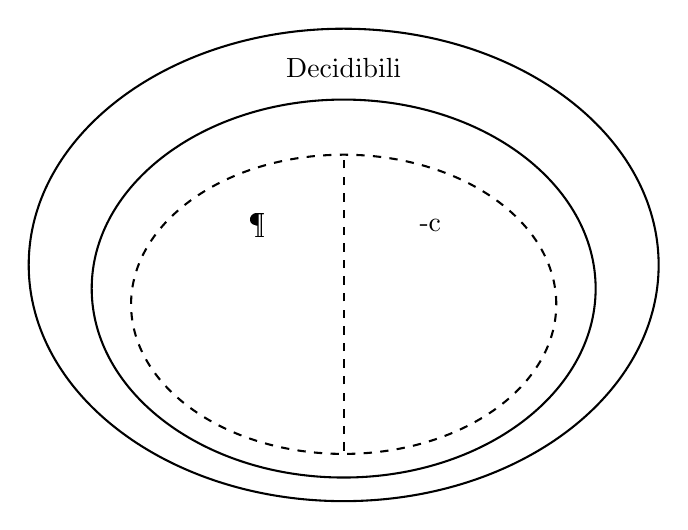
\begin{tikzpicture}[line width=0.75pt]
	\draw         (0,0)      ellipse (4cm and 3cm);
	\draw         (0,2.5)    node {Decidibili};
	\draw         (0,-0.3)   ellipse (3.2cm and 2.4cm);
	\draw         (0,1.7)    node {\NP};
	\draw[dashed] (0,-0.5)   ellipse (2.7cm and 1.9cm);
	\draw         (-1.1,0.5) node {\P};
	\draw         (1.1,0.5)  node {\NP-c};
	\draw         (1.3,-0.8) node {\Sat};
	\draw[dashed] (0,-2.36) -- (90:1.4);
\end{tikzpicture}

	\caption{Classi di complessità strutturale.}
	\label{fig:structcomplclass}
\end{figure}



\section{Problemi di ottimizzazione}

\begin{defin}[problema di ottimizzazione]
	Un problema di ottimizzazione è una tupla $\Pi=\tuple{I,\amm,c,T}$, con:
	\begin{itemize}
		\item $I_\Pi\in\set{0,1}\star$ è l'insieme degli input;
		\item $\amm_\Pi: I_\Pi\to2^{2\star}\setminus\set{\emptyset}$ è l'insieme delle soluzioni ammissibili;
		\item $c_\Pi:I_\Pi\times 2\star\to\Q^+$ è la funzione obiettivo (o di costo), che associa un valore a un output per un dato input;
		\item $T_\Pi \in\set{\MIN,\MAX}$ è il tipo di ottimizzazione: l'obiettivo è minimizzare la funzione obiettivo se $T_\Pi=\MIN$ e massimizzarla se $T_\Pi=\MAX$.
	\end{itemize}
\end{defin}

\begin{examp}
	\MaxSat è la versione di ottimizzazione di \Sat. Data una formula logica in forma normale congiuntiva, le soluzioni ammissibili sono i possibili assegnamenti delle variabili e la funzione obietivo è uguale al numero di clausole rese vere. È naturalmente un problema di massimo.
\end{examp}

\begin{defin}[soluzione ottima]
	Dato un problema di ottimizzazione $\Pi$, e $x\in I_\Pi$, una soluzione $y\star(x)\in\amm(x)$ è ottima se e solo se $\forall \bar y\in\amm(x)_\Pi$:
	\begin{equation*}
		c_\Pi(x,y\star(x))
		\begin{cases}
			\geq c_\Pi(x,\bar y) \qquad & T_\Pi=\MAX \\
			\leq c_\Pi(x,\bar y) \qquad & T_\Pi=\MIN
		\end{cases}
	\end{equation*}
\end{defin}

\begin{examp}
	\MaxSat è la versione di ottimizzazione di \Sat. Data una formula logica in forma normale congiuntiva, le soluzioni ammissibili sono i possibili assegnamenti delle variabili e la funzione obietivo è uguale al numero di clausole rese vere. È naturalmente un problema di massimo:
	\popt{\MaxSat}
	{Formule booleane in forma normale congiuntiva}
	{$\N$}
	{Determinare il numero massimo di clausole che si possono rendere vere}
	{Assegnamenti di valori di verità}
	{$\MAX$}
	{Numero di clausole rese vere}
\end{examp}


\subsection{Approssimazioni}
\begin{defin}[rapporto di approssimazione]
	Dati $x\in I_\Pi, y\in\amm_\Pi(x)$, il rapporto di approssimazione $R_\Pi(x,y)$ della soluzione $y$ per input $x$ è:
	\begin{equation*}
		R_\Pi(x,y):=\max\set{\frac{c_\Pi(x,y)}{c_\Pi(x,y\star(x))},\frac{c_\Pi(x,y\star(x))}{c_\Pi(x,y)}}
	\end{equation*}
\end{defin}
\noindent Il rapporto di approssimazione è un numero maggiore o uguale a $1$ e indica un'approssimazione tanto buona quanto più è vicino a $1$. Equivalentemente:
\begin{equation*}
	R_\Pi(x,y)=\begin{cases}
		\dfrac{c_\Pi(x,y)}{c_\Pi(x,y\star(x))} \qquad & T_\Pi=\MIN \\[3ex]
		\dfrac{c_\Pi(x,y\star(x))}{c_\Pi(x,y)} \qquad & T_\Pi=\MAX
	\end{cases}
\end{equation*}

\begin{examp}
	Quando $R_{\Pi}=1$, la soluzione $y$ è ottima. Se $R_{\Pi} = 2$, il costo di $y$ è il doppio del costo di $y^*(x)$ per un problema di minimo, o la metà per un problema di massimo.
\end{examp}
Se si riesce a dimostrare che un algoritmo per un problema di ottimizzazione trova, per ogni input $x$, una soluzione tale che $R(x,y(x))\leq\alpha$, si dice che l'algoritmo è $\alpha$-approssimante.



\subsection{Classi per problemi di ottimizzazione}
Per i problemi di ottimizzazione, si estendono i concetti che definiscono le classi \P e \NP per i problemi di decisione, risultando nelle classi \PO e \NPO.
\begin{defin}[\PO]
	PO è la classe dei problemi di ottimizzazione $\Pi$ in cui $y\star(x)$ è calcolabile in tempo polinomiale deterministico $\forall x\in I_\Pi$.
\end{defin}

\begin{defin}[\NPO]
	Dato un problema di ottimizzazione $\Pi$, $\Pi\in\text{NPO}$ se e solo se:
	\begin{itemize}
		\item $I_\Pi\in P$, ossia si può decidere l'appartenenza di un valore agli input di $\Pi$ in tempo polinomiale;
		\item esiste un polinomio $Q$ tale che
		      \begin{itemize}
			      \item $\forall x\in I_\Pi \forall y\in\amm_\Pi(x): \len y\leq Q(\len x)$, ossia le soluzioni ammissibili non superano in lunghezza un polinomio nella lunghezza di $x$;
			      \item $\forall x\in I_\Pi \forall y\in 2\star:$ se $\len y\leq Q(\len x)$ si può decidere se $y\in\amm_pi(x)$ in tempo polinomiale in $\len x$.
		      \end{itemize}
		\item $c_\Pi$ è calcolabile in tempo polinomiale.
	\end{itemize}
\end{defin}
Il concetto di nondeterminismo applicato a \NPO è individuato nella possibilità di scegliere nondeterministicamente una stringa $y$ tale che $\len y\leq Q(\len x)$, controllare in tempo polinomiale se è una soluzione valida e calcolare in tempo polinomiale il suo obiettivo. Tale obiettivo è ottimo se si suppone che la scelta nondeterministica sia corretta.


\subsection{Problema di decisione associato e \texorpdfstring{\NPO}{NPO}-completezza}
Si può associare a un problema di ottimizzazione un problema di decisione:
\begin{defin}
	Dato un problema di ottimizzazione $\Pi$, si definisce il problema di decisione $\hat\Pi$, dove:
	\begin{itemize}
		\item $I_{\hat\Pi}=I_\Pi\times\N$
		\item $(x,k)$ ha output $1$ se e solo se
		      \begin{equation*}
			      \begin{cases}
				      c_\Pi(x,y\star(x))\leq k \quad & \text{se } T_\Pi=\MIN \\
				      c_\Pi(x,y\star(x))\geq k \quad & \text{se } T_\Pi=\MAX
			      \end{cases}
		      \end{equation*}
	\end{itemize}
\end{defin}
Il problema di decisione risponde quindi alla domanda: "nel problema di ottimizzazione, è possibile fare meglio di $k$?".

\begin{theorem}
	Sia $\Pi$ un problema di ottimizzazione.
	\begin{enumerate}[(a)]
		\item \label{itm:ott:hatpi:po}$\Pi\in\PO \impl\hat\Pi\in\P$
		\item \label{itm:ott:hatpi:npo}$\Pi\in\NPO \impl\hat\Pi\in\NP$
	\end{enumerate}
\end{theorem}
\begin{proof}
	\ref{itm:ott:hatpi:po} Dato un input $(x,k)$ per $\hat\Pi$, un algoritmo polinomiale per $\Pi$ (che esiste in quanto $\Pi\in\PO$) determina la soluzione ottima per $\Pi$ e restituisce $1$ se essa è migliore di $k$, o $0$ altrimenti.

	% TODO
	\ref{itm:ott:hatpi:npo} \dots
\end{proof}

\begin{defin}[problema \NPO-completo]
	Un problema $\Pi$ è \NPO-completo se appartiene a \NPO ed è tale che $\hat\Pi$ è \NP-completo.
\end{defin}

\begin{theorem}
	Se $\Pi$ è NPO-completo, $\P\neq \NP\impl\Pi\notin\PO$
\end{theorem}
\begin{proof}
	Sia $\Pi$ \NPO-completo e $\P\neq\NP$.	Per assurdo supponiamo che $\Pi\in\PO$. Supponiamo senza perdita di generalità che $T_\Pi=\MAX$. Allora su input $(x,k)\in I_\Pi\times\N$:
	\begin{itemize}
		\item si calcola $y\star(x)$ in tempo polinomiale (essendo $\Pi\in\PO$)
		\item si calcola $c(x,y\star(x))$ in tempo polinomiale
		\item se $c(x,y\star(x))\geq k$ si dà output positivo, altrimenti si dà output negativo
	\end{itemize}
	Si è trovato un algoritmo polinomiale per decidere $\hat\Pi$, il che per ipotesi è assurdo.
\end{proof}

\begin{theorem}
	\MaxSat è \NPO-completo
\end{theorem}
\begin{proof}
	% TODO: elaborare
	$\MaxSat\in\NPO$.

	Dimostriamo che $\widehat{\MaxSat}$ è NP-completo riducendo \Sat ad esso. Dato un input $x$ per \Sat, sia $(x,k)$ l'input per $\widehat{\MaxSat}$, dove $k$ il numero di clausole in $x$, calcolabile in tempo polinomiale. Una formula è soddisfacibile se e solo se il numero di clausole soddisfacibili è maggiore o uguale (cioè uguale) del numero di clausole, quindi l'output di $\widehat{\MaxSat}$ su $(x,k)$ è uguale all'output di $\Sat$ su $x$.
\end{proof}


\subsection{Classi per problemi approssimabili}

\begin{defin}[\gAPX{$\gamma$}]
	\gAPX{$\gamma$}, con $\gamma\geq1$, è l'insieme dei problemi di ottimizzazione $\Pi$ tali che esiste un algoritmo che dato $x\in I_\Pi$ trova una soluzione $y\in\amm_\Pi(x)$ in tempo polinomiale tale che $R_\Pi(x,y)\leq \gamma$.
\end{defin}
\begin{defin}[\APX]
	\begin{equation*}
		\APX=\bigcup_{\gamma\geq1} \gAPX{\gamma}
	\end{equation*}
\end{defin}

% TODO: definizioni da rivedere
\begin{defin}
	\PTAS (Polynomial Time Approximation Scheme) è la classe di problemi di ottimizzazione $\Pi$ tali che esiste un algoritmo che dato $x\in I_\Pi$ e $\varepsilon>1$, trova in tempo polinomiale in $\len x$ un $y\in\amm_\Pi(x)$ con $R_\Pi(x,y)\leq\varepsilon$.
\end{defin}
\noindent Si noti che il tempo è polinomiale in $\len x$ ma non necessariemente in $\varepsilon$.
\begin{defin}
	\FPTAS è la classe dei problemi di \PTAS tali che l'algoritmo caratteristico ha tempo polinomiale sia in $\len x$ sia in $1/\varepsilon$.
\end{defin}


\begin{figure}
	\centering
	\tikzset{every picture/.style={line width=0.75pt}}
	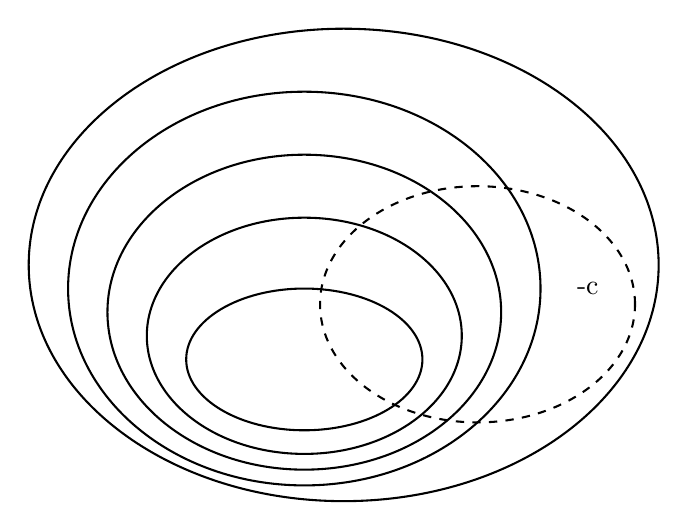
\begin{tikzpicture}[line width=0.75pt]
	\node at (-1.1,2.5) {\NPO};
	\draw (0,0) ellipse (4cm and 3cm);
	\node at (-1.1,1.7) {\APX};
	\draw (-0.5,-0.3) ellipse (3cm and 2.5cm);
	\node at (-1.1,0.9) {\PTAS};
	\draw (-0.5,-0.6) ellipse (2.5cm and 2cm);
	\node at (-1.1,0) {\FPTAS};
	\draw (-0.5,-0.9) ellipse (2cm and 1.5cm);
	\node at (-1.1,-1.1) {\PO};
	\draw (-0.5,-1.2) ellipse (1.5cm and 0.9cm);
	\node at (3.1,-0.3) {\NPO-c};
	\draw[dashed] (1.7,-0.5) ellipse (2cm and 1.5cm);
\end{tikzpicture}

	\caption{Rappresentazione insiemistica delle classi di complessità.}
	\label{fig:compsets}
\end{figure}
